\section{Testing Settings and Generated Artifacts}
\label{sec:landscape}
Figure~\ref{fig:literature-map} maps representative work to testing settings and generated artifacts. The mechanism labels identify selected operations discussed below; they are illustrative assignments rather than exhaustive coding or publication counts.

\begin{figure}[t]
\centering
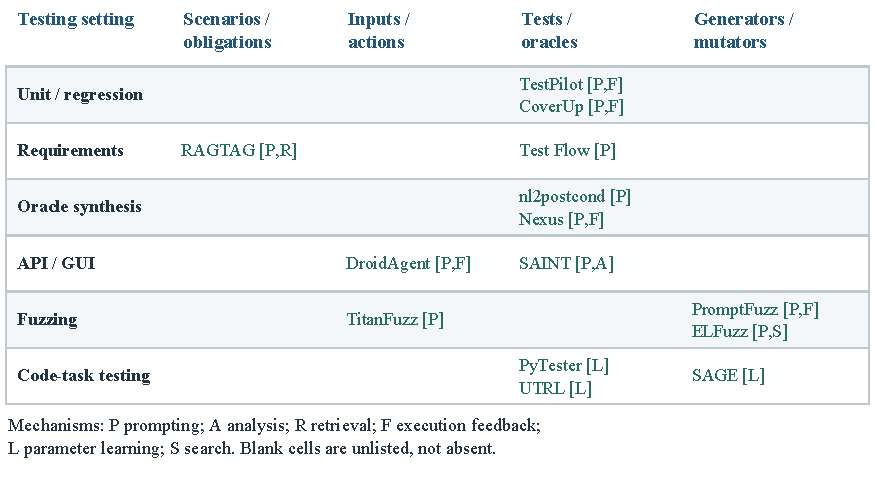
\includegraphics[width=\linewidth]{figures/literature-map.pdf}
\caption{A representative literature map, based on the methods discussed in this section~\cite{U01,U05,R01,R03,O01,O03,A02,A03,F01,F05,F06,T01,T02,T08}. A setting can produce several kinds of artifacts, and mechanisms can be combined. Blank cells indicate no example selected for display.}
\Description{A matrix locates representative methods across six testing settings and four artifact families. Mechanism labels distinguish prompting, analysis, retrieval, feedback, parameter learning, and search. Empty cells do not establish a research gap.}
\label{fig:literature-map}
\end{figure}

\subsection{Unit Tests and Repository Context}
Unit-test generation is the most visible setting in the reviewed collection. The task appears local because the target is a function or method, but executable tests depend on surrounding types, imports, initialization, and test conventions. AthenaTest established an earlier transformer-based approach that uses focal context and supervised code--test data~\cite{U11}. TestPilot combines function information and documentation with execution-based repair~\cite{U01}, while ChatUniTest organizes generation, validation, and repair into a framework~\cite{U02}. These approaches illustrate the transition from generating a plausible test body to constructing an executable artifact in its environment.

Repository context becomes particularly important when the target cannot be instantiated in isolation. CITYWALK uses project-dependency awareness and language-specific knowledge for C++ test generation~\cite{U08}. Its setting highlights why results on standalone functions do not directly characterize class construction, linking, fixtures, or external dependencies. In regression-oriented systems such as TestGen-LLM, existing tests additionally supply conventions and a baseline to improve~\cite{U07}. These conventions can make generated tests easier to integrate, although their behavioral assumptions still require interpretation.

\subsection{Requirements, Scenarios, and Acceptance Tests}
Requirements-driven generation begins with intended behavior expressed independently of an executable test. RAGTAG retrieves domain information to generate test scenarios from natural-language requirements~\cite{R01}. Multi-step generation of system-level test specifications uses intermediate artifacts to structure this transformation~\cite{R02}. Both settings expose an important distinction: producing a useful test design and producing a runnable script are separate accomplishments, with different evaluation methods and human responsibilities.

An industrial acceptance-testing study makes this separation explicit. AutoUAT transforms user stories into Gherkin scenarios, while Test Flow uses those scenarios and page HTML to construct Cypress scripts~\cite{R03}. Information access changes between stages. The scenario can be judged against a user story; the script also needs knowledge of concrete page structure. APITestGenie similarly combines requirements and API specifications to generate web API tests~\cite{R04}. These pipelines suggest that traceability should connect the requirement, the scenario, the executable actions, and the assertion, so that a failure can be attributed to the appropriate transformation.

\subsection{Oracles, Postconditions, and Metamorphic Relations}
Oracle generation isolates the part of a test that decides whether behavior is acceptable. TOGA generates exception and assertion oracles using a neural approach~\cite{O04}. Its subsequent large-scale evaluation and replication work demonstrates the importance of examining oracle generation under changed evaluation conditions~\cite{O05}. An oracle should therefore be assessed by the behavior it accepts and rejects, in addition to whether it resembles a developer-written assertion.

Postconditions and metamorphic relations broaden the oracle representation. The nl2postcond work translates natural-language intent into executable method postconditions~\cite{O01}. Work on executable metamorphic relations derives relations from requirements and API specifications~\cite{O02}. A relation can test consistency across executions when predicting one exact output is difficult. Its applicability conditions are part of its meaning: a plausible transformation can be invalid for inputs that violate an unstated precondition. Thus, generating the relation and establishing its domain of validity remain distinct tasks.

Nexus uses execution-grounded multi-agent processes for oracle synthesis~\cite{O03}, and CANDOR incorporates multi-agent consensus into end-to-end JUnit generation~\cite{O06}. These approaches combine test construction and oracle review. Their interaction patterns can expose contradictions, but the source of behavioral evidence still determines what agreement establishes. Agreement among agents or with candidate executions must be interpreted relative to the requirements being tested.

\subsection{API and GUI Interaction Sequences}
For APIs and GUIs, test generation must maintain state across actions. An endpoint can require a resource identifier returned by an earlier request; a GUI action can depend on a screen reached through navigation. AutoRestTest combines LLM support with multi-agent reinforcement learning for REST API testing~\cite{A01}. SAINT uses program analysis and LLM-based agents for service-level integration tests~\cite{A02}. The relevant artifact is therefore a coordinated interaction sequence, including dependencies between operations, rather than a collection of independent input values.

DroidAgent and GPTDroid apply LLM reasoning to mobile GUI exploration and interaction~\cite{A03,A04}. Here, observations and actions are interleaved: the next action depends on the current interface. Reaching a screen demonstrates exploration; checking that the screen implements a requirement additionally needs an oracle. This distinction also affects replay. A sequence generated through adaptive interaction may need stable selectors, state initialization, and checkpoints before it becomes a repeatable regression test.

\subsection{Fuzzing Inputs and Infrastructure}
Fuzzing gives the LLM a different role. TitanFuzz and FuzzGPT generate programs for testing deep-learning libraries, with the latter emphasizing edge cases~\cite{F01,F02}. Fuzz4All uses LLMs in a broader fuzzing framework~\cite{F03}. These methods exploit the model's ability to produce structured inputs while relying on execution and external failure detectors to identify anomalies.

The generated object can also be an input generator. ChatAFL extracts protocol-related information to support grammar construction and message-sequence exploration~\cite{F04}. PromptFuzz generates fuzzing drivers~\cite{F05}; ELFuzz searches over synthesized fuzzers~\cite{F06}; Bulbasaur generates customized mutators using branch-oriented information~\cite{F07}. This progression changes the cost model because one generated artifact can produce many executions. A survey that records only the number of LLM-generated test cases would miss both the reuse and the contribution of the conventional fuzzing engine.

\subsection{Bug Reproduction and Tests for Code Generation}
LIBRO generates bug-reproducing tests from natural-language reports~\cite{G01}. SWT-Bench evaluates test generation in the context of real-world fixes~\cite{B03}. These settings provide a particular behavioral distinction: the test should expose the issue in a buggy version and accept a fixed version. Reproducing a known failure and discovering an unknown defect are related capabilities but use different information.

Generated tests also influence which code is selected or how it is repaired. CodeT uses generated tests to help choose among candidate programs~\cite{T10}, UTGen learns tests for automated debugging~\cite{T05}, and CodeRM scales test generation for code reward modeling~\cite{T06}. TiCoder introduces user feedback on tests to clarify intent during code generation~\cite{T11}. In all four cases, the downstream outcome depends on both the generator and the consumer of its tests. A useful survey must therefore retain test-level measurements alongside code-selection or repair outcomes.
